\section{Class diagram}

In this section, you will find the class diagram of our current implementation. As you can see 
our current implementation has grown a lot during this sprint, thanks to the addition of various classes. \newline

The participant class had some attribute added and was linked to the new court and pair class so we could which court and pair belongs to who. The pair class was then linked to the new class extra which now allow us to calculate the total price of the inscription. A tournoi class has been added to link the pair creation to a tournoi in particular. \newline

Of course, since this diagram is bound to change, we will update it in the following reports.

\begin{figure}[!ht]
	\centering
	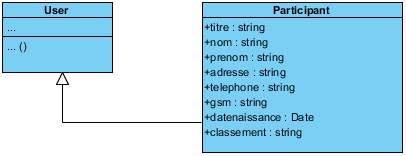
\includegraphics[width=0.8\linewidth]{classdiagram.png}
	\caption{Class diagram of our current implementation}
	\label{fig:length_eight_mouse}
\end{figure}
\FloatBarrier
